\section{Near-Ballistic Transfers between the Earth-Moon and Sun-Earth Systems}
While both categories of trajectories travel through the Sun-Earth CR3BP region, only those with an
intermediate staging orbit have a constrained path. For these trajectories, the Earth-Moon unstable
manifold arc, propagated under the Sun-Earth CR3BP dynamics once it reaches the lunar sphere of
influence, must intersect with a stable manifold arc from the Sun-Earth staging $L_{2}$ halo orbit.
An unstable manifold arc from this orbit is then used to depart the Sun-Earth system (compared to
the more direct transfer type that uses the Earth-Moon manifold to depart the system). Kakoi
developed a design methodology for maneuver-free transfers between orbits in the two systems,
treating them as non-coplanar, where the required respective initial orientations of the three
bodies (the Sun, Earth, and Moon) are represented by angles and the interface between the CR3BP
systems occurs at the intersection of the manifolds\cite{Kakoi:2014,Kakoi:2015}. This methodology
inspired the approach used in this investigation, where the orientations are determined by a
specified epoch date and the two systems interface prior to the arc intersection.

\subsection{Methodology}
To find a connection between the orbits in the two different CR3BP systems, discretized arcs of the
manifold surface of the Earth-Moon departure orbit are propagated to the SoI of the Moon, as
defined in \cref{eq:blendedSoI}. At this distance from the Moon, its gravitational influence
becomes negligible compared to those of the Earth and the Sun. At this interface of the two CR3BP
systems, the Earth-Moon barycentric rotating frame state of each arc is transformed to a Sun-Earth
barycentric rotating frame state by rotation to the Earth-centered Ecliptic J2000 inertial frame
and back as described in Section 2.5.2. This rotation is dependent on the epoch date when the state
reaches the SoI, as this determines the relative orientations of the celestial bodies. While the
orientations change slightly month-to-month due to the different planes, the transfer
characteristics tend to repeat each month, so this study only investigates transfers during January
2026\cite{Parker:2013}.

Note that although these states all had the same Earth-Moon Jacobi constant
value, now that they are in the Sun-Earth system, their Jacobi constant values will vary. Since
these new values will remain constant as the states are now propagated with the Sun-Earth CR3BP
equations of motion, it is necessary that the Jacobi constant of the Sun-Earth staging halo lies
within that range of values. The manifold arcs are now propagated until they reach the manifold
intersect hyperplane, chosen as an angle measured from the $x$-axis in the Sun-Earth rotating
frame. According to Kakoi, hyperplane angles between $-\ang{85}$ and $\ang{70}$ are desirable for
transfers between Earth-Moon $L_{2}$ and Sun-Earth $L_{2}$ orbits, with $\ang{-80}$ being used in
this investigation\cite{Kakoi:2015}. At the same time, the discretized stable manifold surface from
the Sun-Earth $L_{2}$ halo orbit is propagated to the same hyperplane, as shown in
\cref{fig:hyperplane}.

\begin{figure}[ht]
    \centering
    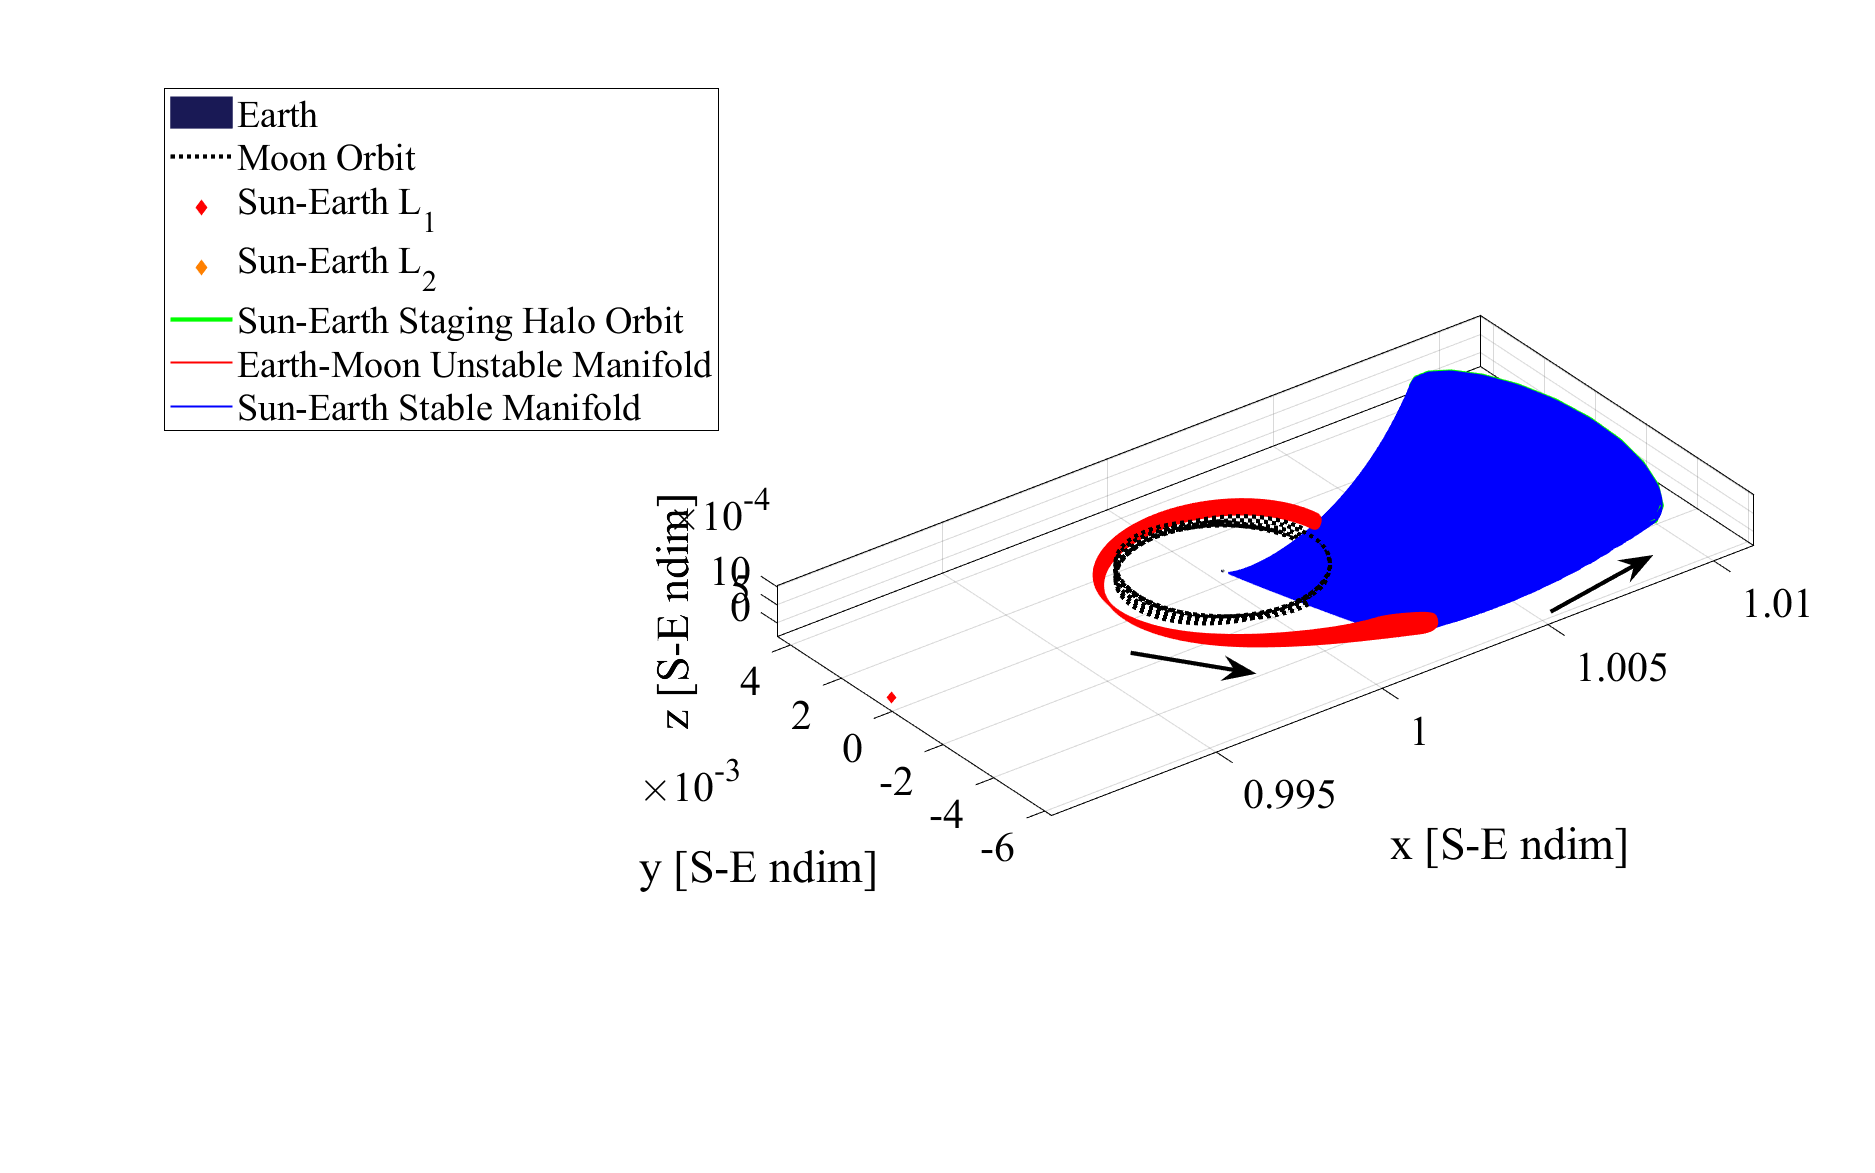
\includegraphics[width=0.9\textwidth]{figures/Hyperplane.pdf}
    \caption{Earth-Moon and Sun-Earth manifolds intersecting at the hyperplane.}
    \label{fig:hyperplane}
\end{figure}

At the hyperplane, mappings of both sets of manifold arcs are used to form phase plots that inform
the transfer initial guess selection. Following Kakoi's approach, the plots represent $\xdot$ vs.
$x$, $z$ vs. $x$, and $\zdot$ vs. $z$. The $y$-value is defined by the $x$-value and the hyperplane
angle, while the $\ydot$-value is determined by the Jacobi constant\cite{Kakoi:2015}. A black dot
along the Earth-Moon manifold curve is also used to denote the arc that matches the Sun-Earth
manifold in Jacobi constant. The two sets of manifold arcs form curves on the plots and the goal is
to find an intersection between the curves in all three phase plots that occurs at the black point.
\cref{fig:phasePlots} shows an example of these phase plots, where the red curve is the unstable
Earth-Moon manifold and the blue curve is the stable Sun-Earth manifold. Note that there are two
black markers representing two arcs that match the Sun-Earth Jacobi constant. The initial epoch of
the Earth-Moon manifold departure, the hyperplane angle, and the Sun-Earth halo Jacobi constant can
all be varied to shift the curves on the phase plots and find an intersection; Kakoi provides some
guidelines on how to do so\cite{Kakoi:2015}. Once a suitable point is determined, like the black
circle marker in \cref{fig:phasePlotsIntersect}, this information can be used to generate an
initial guess for the transfer between the systems, shown in .

\begin{figure}[ht]
    \centering
    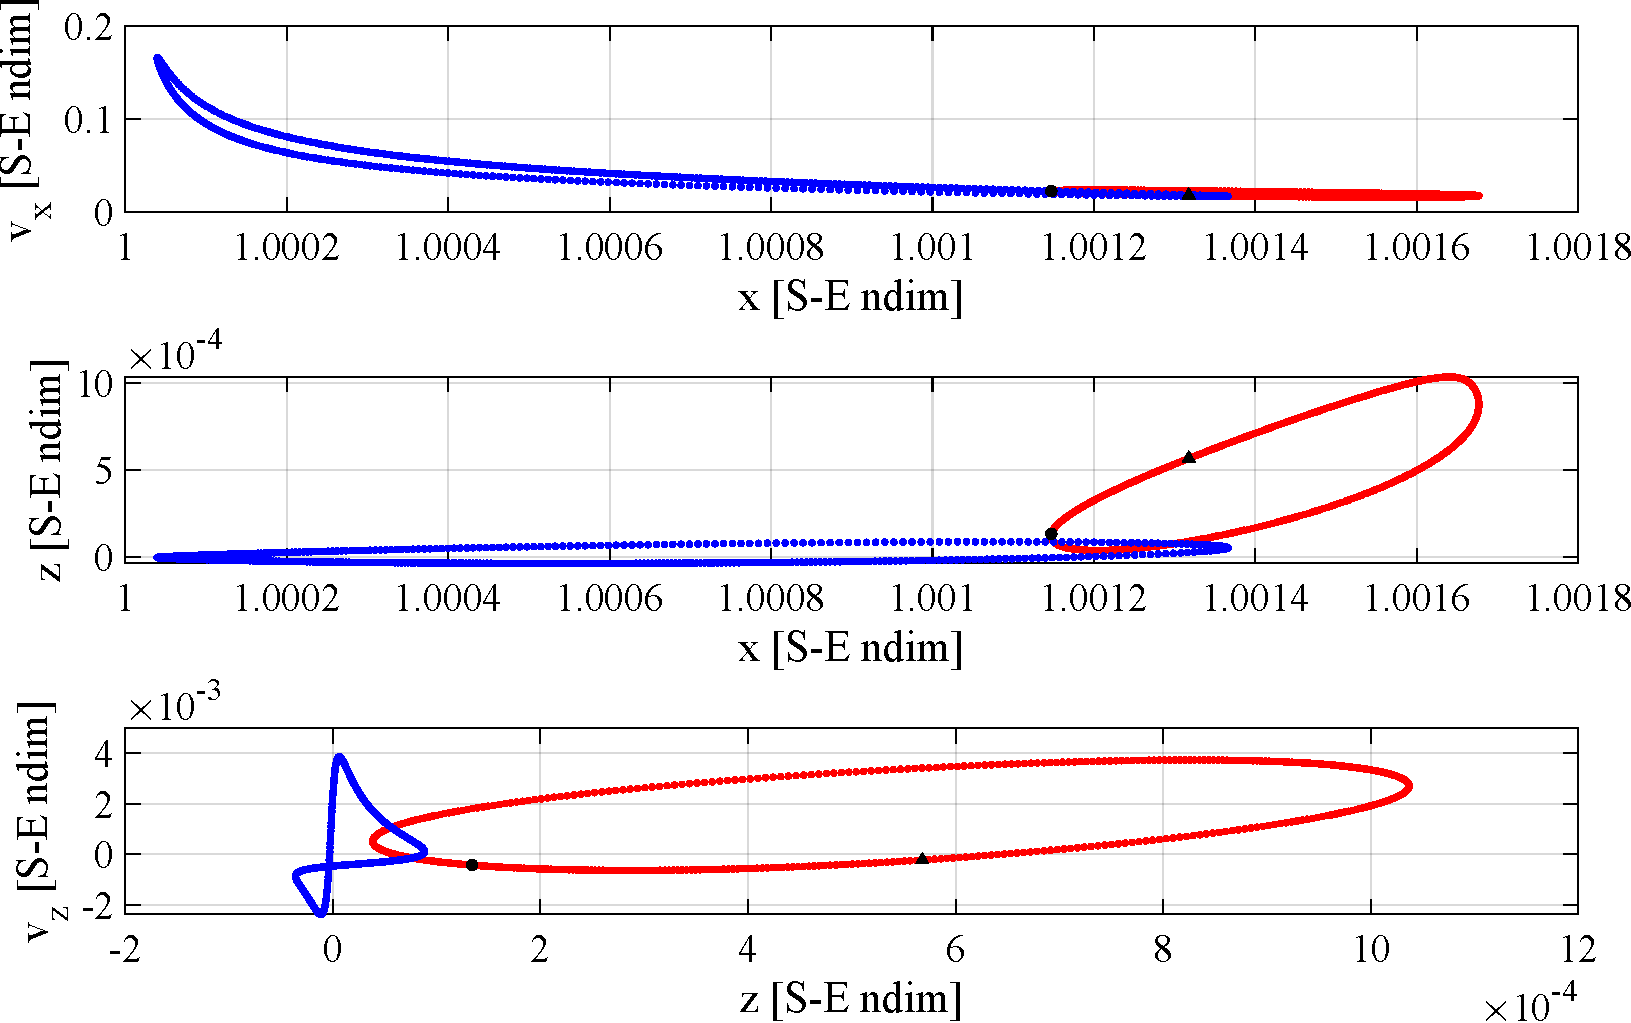
\includegraphics[width=0.75\textwidth]{figures/PhasePlots.pdf}
    \caption{The hyperplane phase plots for \cref{fig:hyperplane}.}
    \label{fig:phasePlots}
\end{figure}

\begin{figure}[ht]
    \centering
    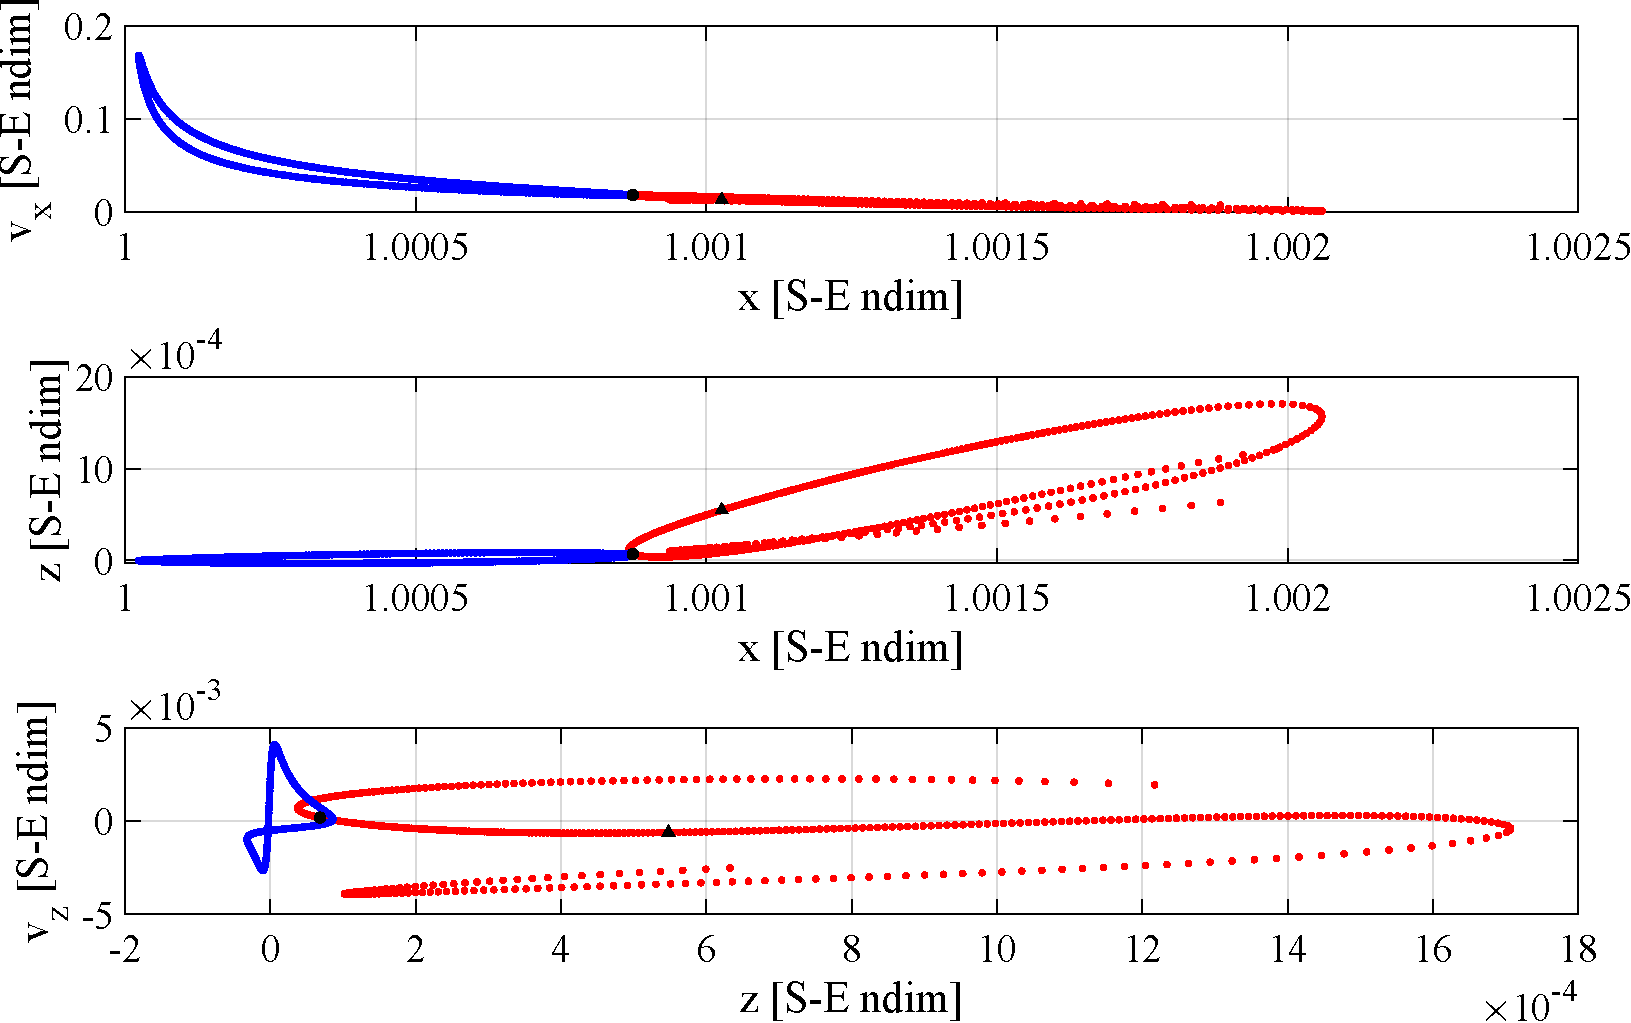
\includegraphics[width=0.75\textwidth]{figures/PhasePlotsIntersect.pdf}
    \caption{Hyperplane phase plots with a near intersection after varying the parameters.}
    \label{fig:phasePlotsIntersect}
\end{figure}

\subsection{Example}
